\documentclass[aspectratio=169]{beamer}

\usetheme{default}

\usepackage[utf8]{inputenc}
\usepackage[russian]{babel}
\usepackage[OT1]{fontenc}
\usepackage{amsmath}
\usepackage{amsfonts}
\usepackage{amssymb}
\usepackage{graphicx}
\usepackage{etoolbox}
\usepackage{caption}
\usepackage{subcaption}
\captionsetup{compatibility=false}
\usepackage{pifont}
%\usepackage{subfigure}
\usepackage{xcolor}
\usepackage{framed}
\usepackage{empheq}
\usepackage[many]{tcolorbox}
\usepackage{multirow}
\usepackage{tikz}
\usepackage{listings}
\usepackage{tikz}

\definecolor{shadecolor}{cmyk}{0,0,0,1}

\lstset{
	backgroundcolor=\color{lightgray},
	commentstyle=\color{blue},
	frame=single
	breakatwhitespace, 
	language=python, 
	columns=fullflexible, 
	keepspaces, 
	breaklines, 
	tabsize=3, 
	showstringspaces=false, 
	extendedchars=true,
	numbers=left
}

\makeatletter

\setbeamercolor{title}{fg=white}
\setbeamercolor{frametitle}{fg=black}
\setbeamerfont*{title}{family=\sffamily,size=\LARGE}

\setbeamerfont{page number in head/foot}{size=\scriptsize}
\setbeamertemplate{footline}[frame number]
\let\otp\titlepage
\renewcommand{\titlepage}{\otp\addtocounter{framenumber}{-1}}

\setbeamertemplate{background canvas}{%
	\ifnumequal{\c@framenumber}{0}{%
		\vbox to \paperheight{\vfil\hbox to \paperwidth{\hfil
\includegraphics[height=\paperheight]{images/cover.png}\hfil}\vfil}
   }{%
      \ifnumequal{\c@framenumber}{\inserttotalframenumber}{
        \vbox to \paperheight{\vfil\hbox to \paperwidth{\hfil
\includegraphics[height=\paperheight]{images/back.png}\hfil}\vfil}
      }{%
         % Other frames
      }%
   }%
}

\makeatother

\beamertemplatenavigationsymbolsempty

\tcbset{highlight math style={enhanced,colframe=red,colback=white,arc=4pt,boxrule=1pt}}

\usetikzlibrary{shadings,shadows,shapes.arrows}

\newcommand*{\tikzarrow}[2]{%
  \tikz[
    baseline=(A.base),             % Set baseline to the baseline of node content
    font=\footnotesize\sffamily    % Set fontsize of the node content
  ]
  \node[
    single arrow,                  % Shape of the node
    single arrow head extend=5pt,  % Actual width of arrow head
    draw,                          % Draw the node shape
    inner sep=3pt,                 % Separation between node content and node shape
    top color=#1,               % Shading color on top of node
    bottom color=#1,               % Shading color on bottom of node
    % drop shadow                    % Draw a shadow
  ] (A) {#2};%
}

\newcommand{\tikzfancyarrow}[2][2cm]{\tikz[baseline=-0.5ex]\node [arrowstyle=#1] {#2};}
\newcommand*\rot{\rotatebox{90}}

\author{Николай Анохин}
\title{\newline \newline \newline Лекция 5 \\ Классификация и регрессия}

\begin{document}

\begin{frame}[plain]
\titlepage
\end{frame}

\begin{frame}{План занятия}
\tableofcontents
\end{frame}

% ========================================
\section{Задачи классификации и регрессии}
% ========================================

\begin{frame}{}

\begin{center}
\Large Задачи классификации и регрессии

\vspace{1em}

\includegraphics[height=0.7\textheight]{images/omnomnom.jpg}
\end{center}

\end{frame}

\begin{frame}{Классификация: интуиция}

\begin{block}{Задача}
Разработать алгоритм, позволяющий определить класс произвольного объекта из некоторго множества
\begin{itemize}
\item Дана {\it обучающая выборка}, в которой для каждого объекта известен класс
\end{itemize}
\end{block} 

\begin{center}
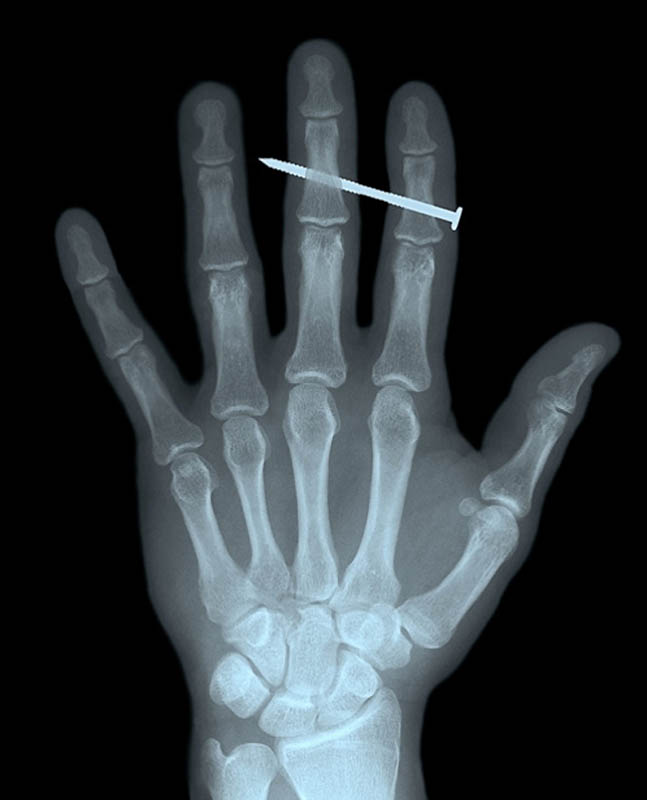
\includegraphics[scale=0.15]{images/xray.jpg}
\end{center}

\end{frame}

\begin{frame}{Регрессия: интуиция}

\begin{block}{Задача}
Разработать алгоритм, позволяющий предсказать числовую характеристику произвольного объекта из некоторого множества
\begin{itemize}
\item Дана {\it обучающая выборка}, в которой для каждого объекта известно значение числовой характеристики
\end{itemize}
\end{block}

\begin{center}
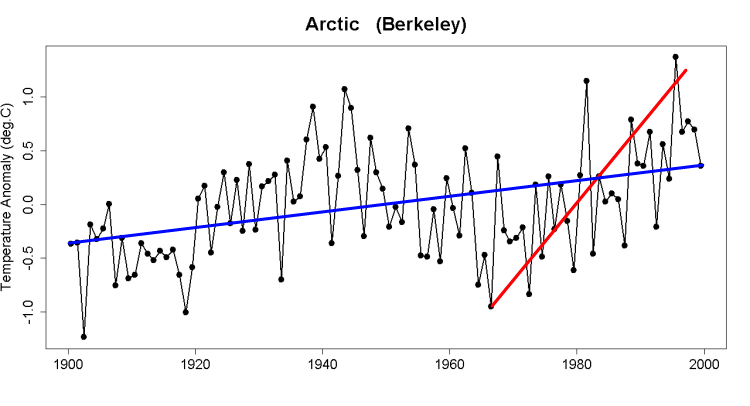
\includegraphics[scale=0.3]{images/kioto.png}
\end{center}

\end{frame}

\begin{frame}{Обучение с учителем / supervised learning}

\vspace{1em}
{\bf Дано.} Признаковые описания $N$ объектов $\mathbf{x} = (x_1, \ldots, x_m) \in \mathcal{X}$, образующие тренировочный набор данных $X$, и значения целевой переменной $y = f(\mathbf{x}) \in \mathcal{Y}$ для каждого объекта из $X$. 

\vspace{1em}
{\bf Найти.} Для семейства параметрических функций 
\[
H = \{h(\mathbf{x, \mathbf{\theta}}) = y: \mathcal{X} \times \Theta \rightarrow \mathcal{Y}\},
\]
найти значение вектора параметров $\theta^*$, такое что $h^*(\mathbf{x}) = h(\mathbf{x}, \theta^*)$ наилучшим образом приближает целевую функцию.

\begin{eqnarray*}
Y & \in & \{C_1, C_2, \ldots, C_N\} \text{ -- задача классификации}  \\
Y & \in & [a, b] \subset \mathcal{R} \text{ -- задача регресии}
\end{eqnarray*}

\end{frame}

\begin{frame}{$L = R + E + O$}

\begin{enumerate}

\item[R] Выдвигаем гипотезу насчет {\bf модели} - семейства параметрических функций вида
\[
H = \{h(\mathbf{x}, \theta) = y: \mathcal{X} \times \Theta \rightarrow \mathcal{Y} \},
\]
которая могла бы решить нашу задачу (represenation)

\item[E] Выбиаем критерий, на основании которого будем оценивать качество предсказания (evaluation)

\item[O] Выбираем наилучшие параметры модели $\theta^*$, используя {\bf алгоритм обучения}
\[
A(X, Y) : (\mathcal{X}, \mathcal{Y})^N \rightarrow \Theta
\]
(optimization)

\item[D] Используя полученную модель $h^*(\mathbf{x}) = h(\mathbf{x}, \theta^*)$, решаем, как классифицировать неизвестные объекты (decision making)

\end{enumerate}

\end{frame}

% ========================================
\section{Некоторые полезные идеи}
% ========================================

\begin{frame}{}

\begin{center}
\Large Некоторые полезные идеи

\vspace{1em}

\includegraphics[width=0.7\textwidth]{images/idea.png}
\end{center}

\end{frame}

\begin{frame}{Цены на недвижимость\footnote{\href{http://www.dcc.fc.up.pt/~ltorgo/Regression/cal_housing.html}{California Housing data set}}}

\begin{center}
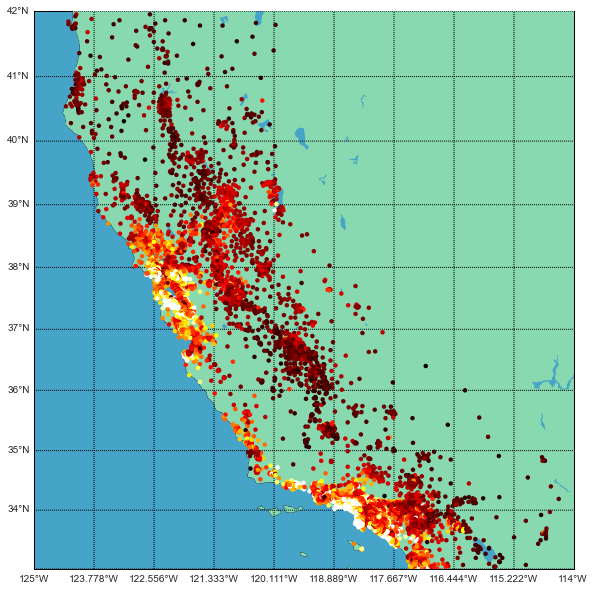
\includegraphics[height=0.6\textheight]{images/large.png} \qquad
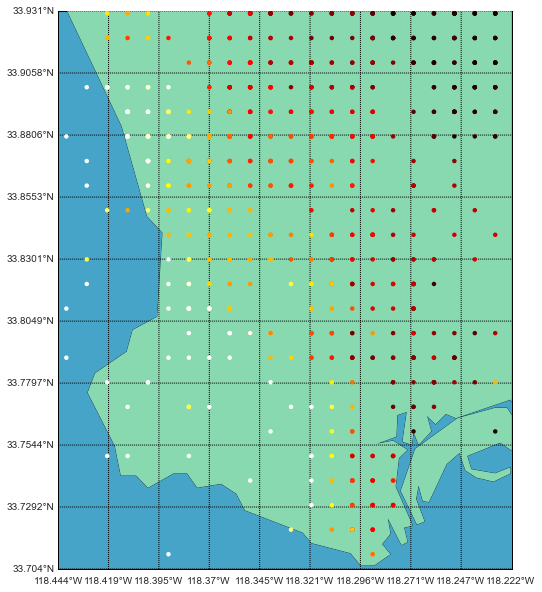
\includegraphics[height=0.6\textheight]{images/map_small.png}
\end{center}

\end{frame}

\begin{frame}{Преобразование данных}

\begin{itemize}
\item Нормализуем широту, долготу
\item Логарифм от целевой переменной
\end{itemize}

\begin{center}
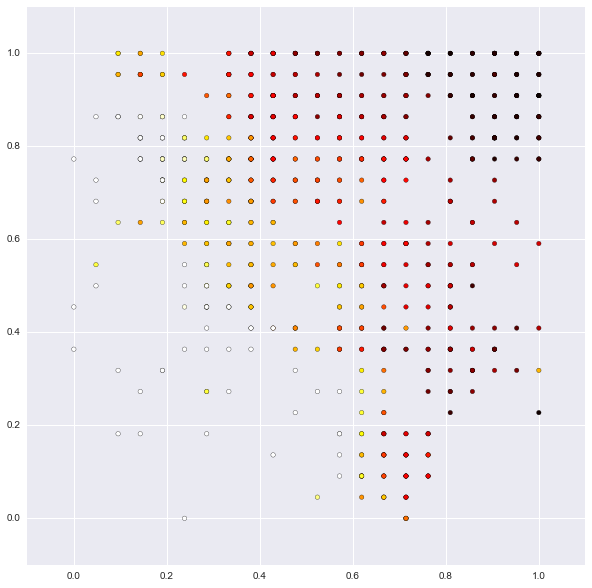
\includegraphics[height=0.5\textheight]{images/small.png} \qquad
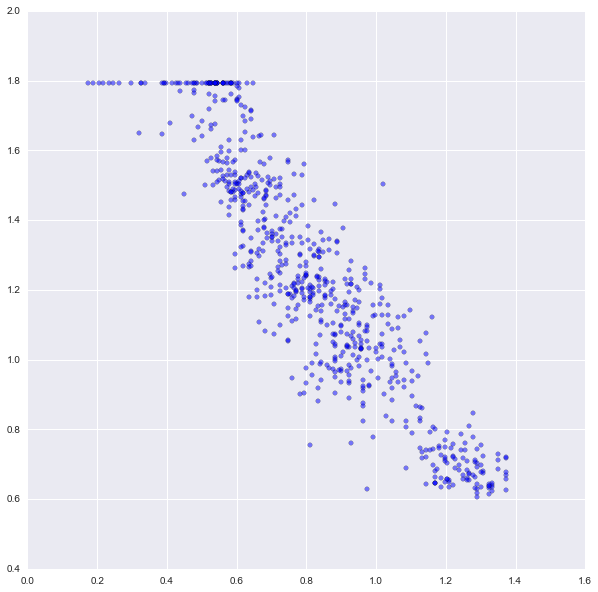
\includegraphics[height=0.5\textheight]{images/ds.png}
\end{center}

\end{frame}

\begin{frame}{Метод ближайших соседей}

K-Nearest Neighbours

\vspace{1em}
Representation:
\[
h(\mathbf{x}) = \frac{1}{K} \sum_{\mathbf{x}_k \in N_K(\mathbf{x})} f(\mathbf{x}_k)
\]

\vspace{1em}
Evaluation: любая

\vspace{1em}
Optimization: не требуется

\end{frame}

\begin{frame}

\begin{center}
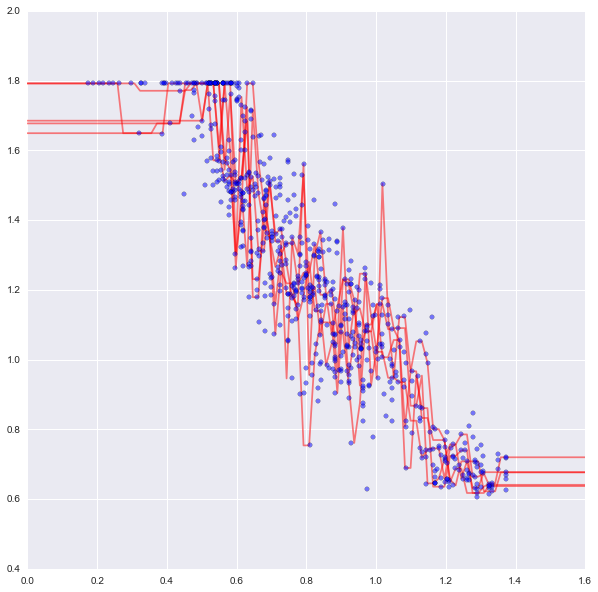
\includegraphics[width=0.3\textwidth]{images/knn1.png}
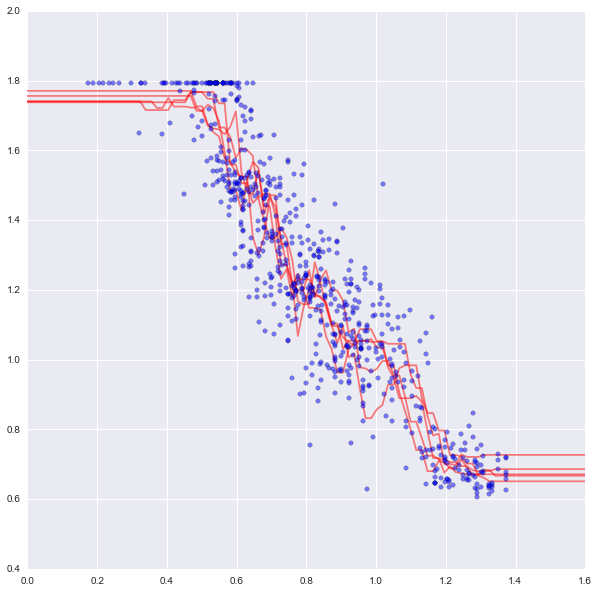
\includegraphics[width=0.3\textwidth]{images/knn5.png}
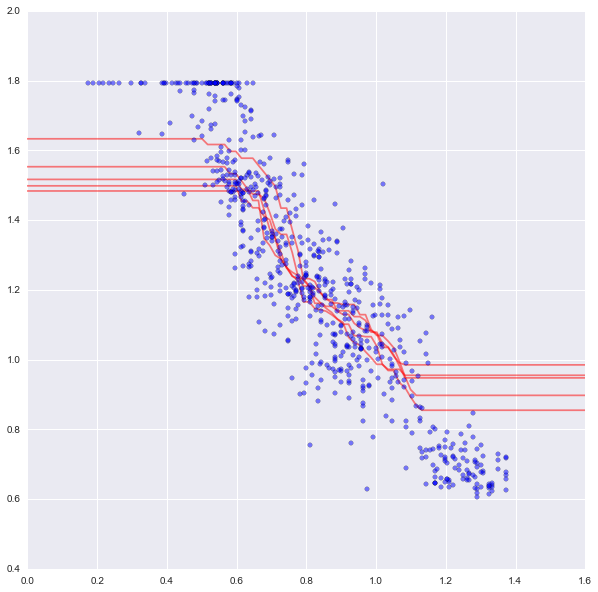
\includegraphics[width=0.3\textwidth]{images/knn30.png}
\end{center}

\end{frame}

\begin{frame}{Классификация с помощью метода ближайших соседей}

\begin{center}
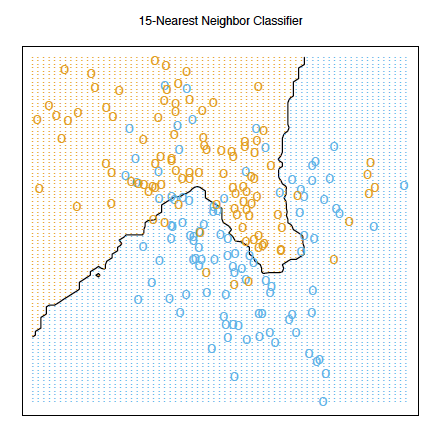
\includegraphics[height = 0.6\textheight]{images/knn_cls.png}
\end{center}

\end{frame}

\begin{frame}{Representation: линейная модель}

Идея: предположить, что искомая функция линейно зависит от признаков
\[
y = h(\mathbf{x}, \mathbf{w}) = \sum_{d=1}^D x_d w_d + w_0 = \mathbf{x}^T \mathbf{w} + w_0
\]
Добавим к $\mathbf{x}$ фиктивный компонент $x_0 = 1$
\[
y = h(\mathbf{x}, \mathbf{w}) = \sum_{d=0}^D x_d w_d = \mathbf{x}^T \mathbf{w},
\]
тогда для всего набора данных
\[
Y = X \mathbf{w}
\]

\end{frame}

\begin{frame}{Evaluation: метод наименьших квадратов}

Идея: выбрать веса так, чтобы сумма квадратов отклонений предсказаний от реальных значений была минимальной
\[
RSS(\mathbf{w}) = \sum_{n=1}^N (y_n - h(\mathbf{x}_n, \mathbf{w}))^2 = \sum_{n=1}^N (y_n - \mathbf{x}_n^T \mathbf{w})^2 \rightarrow \min_{\mathbf{w}}
\]

\end{frame}

\begin{frame}{Optimization: аналитически}

\[
RSS(\mathbf{w}) = (Y - X^T \mathbf{w})^T (Y - X^T \mathbf{w})
\]
\[
\Downarrow
\]
\[
\mathbf{w} = (X^T X)^{-1} X^T Y
\]

\end{frame}

\begin{frame}{Нелинейные зависимости}

Перейдем в новое пространство признаков
\[
\mathbf{x} = (x_1, x_2, \ldots, x_{D})
\]
\[
\downarrow
\]
\[
\mathbf{z} = (x_1, x_2, \ldots, x_D, x_1^2, x_1 x_2, x_1 x_3, \ldots,  x_{D-1} x_D, x_D^2, \ldots)
\]
и сможем приближать сложные нелинейные функции

\end{frame}

\begin{frame}

\begin{center}
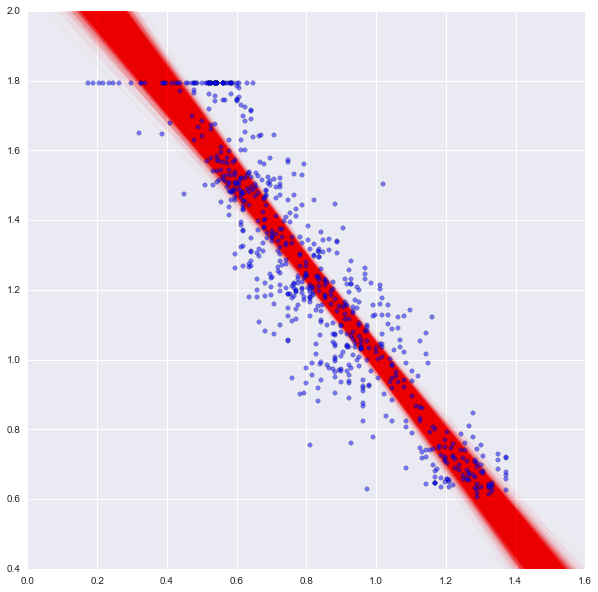
\includegraphics[height=0.55\textheight]{images/lr_fit.png}
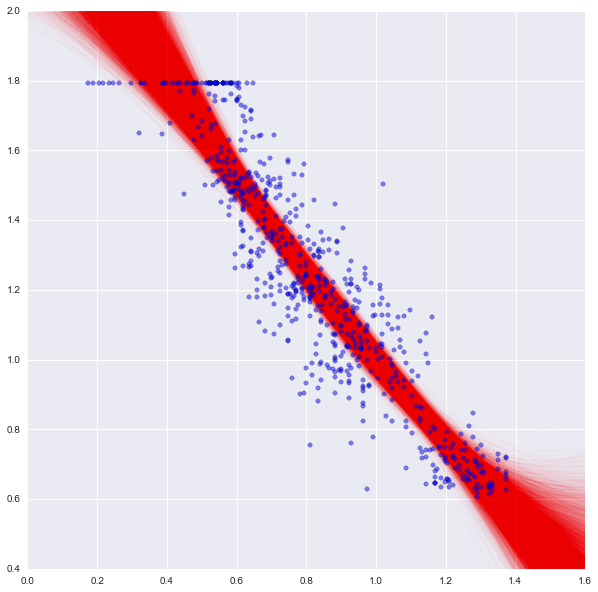
\includegraphics[height=0.55\textheight]{images/qr_fit.png}
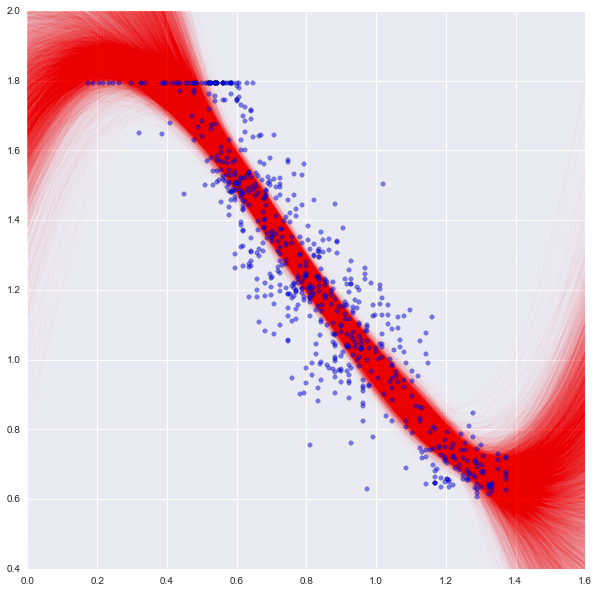
\includegraphics[height=0.55\textheight]{images/tr_fit.png}
\end{center}

\end{frame}

\begin{frame}{Эмпирический риск}

{\bf Функция потерь} $\mathcal{L}(\mathbf{x}, y, \theta)$ - ошибка, которую для данного $\mathbf{x}$ дает модель $h(\mathbf{x}, \theta)$ по сравнению с реальным значением $y$
\vspace{1em}

{\bf Эмпирический риск} -- средняя ошибка на обучающей выборке
\[
Q(X, Y, \theta) = \frac{1}{N} \sum_{n=1}^N \mathcal{L}(\mathbf{x}_n, y_n, \theta)
\]
\vspace{1em}

{\bf Задача} -- найти значение $\theta^*$, минимизирующее эмпирический риск
\[
\theta^* = \theta^*(X, Y) = \text{argmin}_\theta Q(X, Y, \theta)
\]

\end{frame}

\begin{frame}{Некоторые функции потерь}

\begin{itemize}
\item Индикатор ошибки
\[
\mathcal{L}(\mathbf{x}, y, \theta) = 0 \text{\;if\;} h(\mathbf{x}, \theta) = y \text{\;else\;} 1
\]
\item Функция Минковского 
\[
\mathcal{L}(\mathbf{x}, y, \theta) = |y - h(\mathbf{x}, \theta)|^q
\]
Частные случаи: квадратичная $q = 2$, абсолютная ошибка $q = 1$
\item Hinge
\[
\mathcal{L}(\mathbf{x}, y, \theta) = \max(0, 1 - y \times h(\mathbf{x}, \theta))
\]
\item Информационная
\[
\mathcal{L}(\mathbf{x}, y, \theta) = - \log_2 p(y | \mathbf{x}, \theta)
\]
\begin{center}

\end{center}
\end{itemize}

\end{frame}

\begin{frame}{Классификация с помощью метода наименьших квадратов}

\[
\text{Пусть }\mathcal{Y} = \{0, 1\}, \text{ тогда } \begin{cases}
\text{классифицируем 1, если }h^*(\mathbf{x}) \geq 0.5 \\
\text{классифицируем 0, если }h*(\mathbf{x}) < 0.5
\end{cases}
\]

\begin{center}
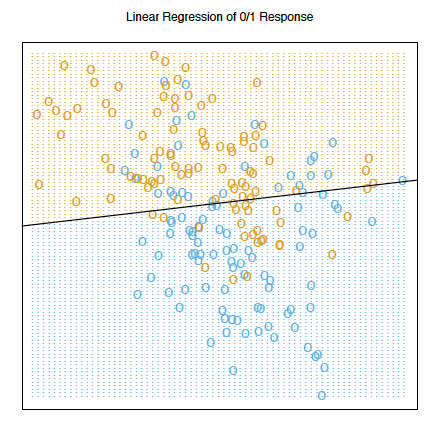
\includegraphics[height=0.5\textheight]{images/lr_cls.png}
\end{center}

\end{frame}

\begin{frame}{Bias-Variance decomposition}

Пусть $y = f(\mathbf{x}) + \varepsilon$, $E[\varepsilon] = 0$, модель $h(\mathbf{x})$

\[
E[(f(\mathbf{x}) + \varepsilon - h(\mathbf{x}))^2] = E[\varepsilon^2] + \left(f(\mathbf{x}) - E[h(\mathbf{x})]\right)^2 + E[(h(\mathbf{x}) -  E[h(\mathbf{x})])^2]
\]
\[
= noise + bias^2 + variance
\]

\begin{center}
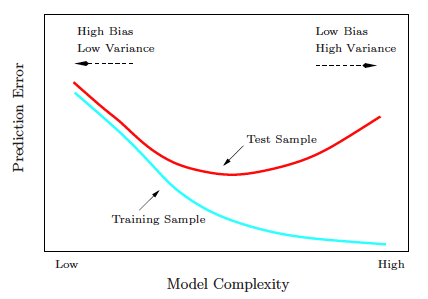
\includegraphics[height=0.5\textheight]{images/bw.png}
\end{center}

Замечание: соотношение сохраняется для других функций потерь

\end{frame}

\begin{frame}{Проблема 1. Переобучение}

Метод наименьших квадратов

\begin{center}
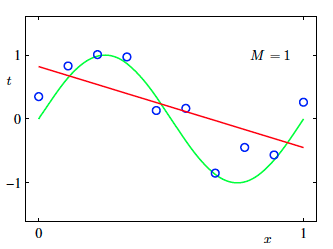
\includegraphics[scale=0.3]{images/m1.png}
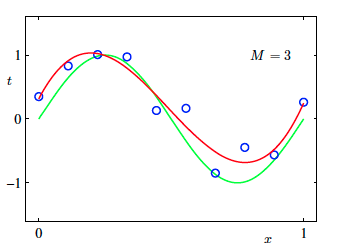
\includegraphics[scale=0.3]{images/m2.png}
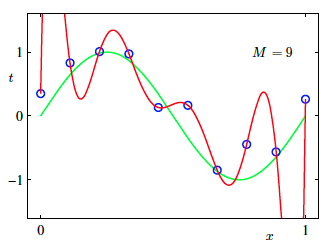
\includegraphics[scale=0.3]{images/m3.png}

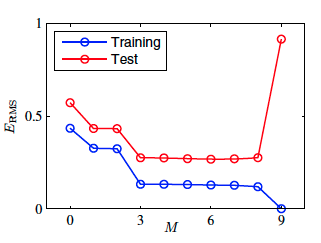
\includegraphics[scale=0.3]{images/of.png}
\end{center}

\end{frame}

\begin{frame}{Проблема 1. Переобучение}

KNN

\begin{center}
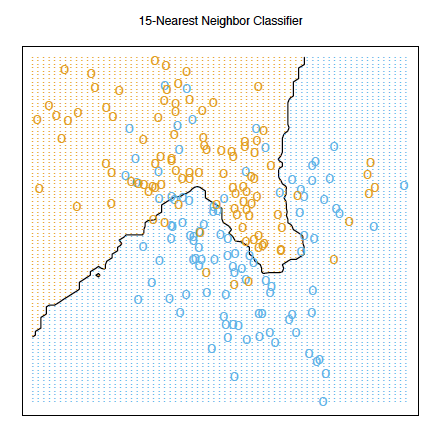
\includegraphics[scale=0.3]{images/knn_cls.png}
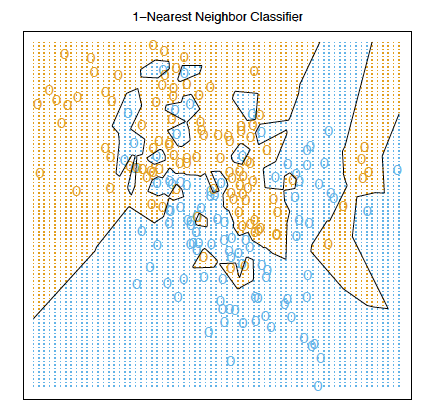
\includegraphics[scale=0.3]{images/knn_cls_1.png}
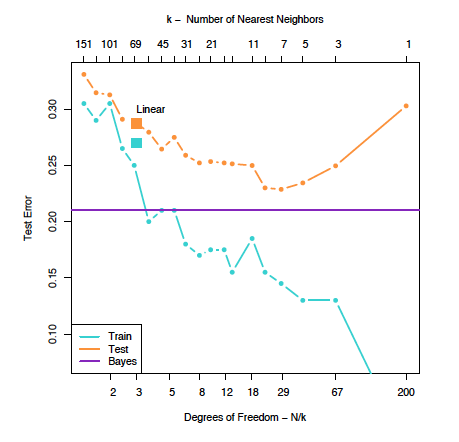
\includegraphics[scale=0.3]{images/knn_tt.png}

\end{center}

\end{frame}

\begin{frame}{Проблема 2. Проклятие размерности\footnote{\href{http://jeremykun.com/2016/02/08/big-dimensions-and-what-you-can-do-about-it/}{Big Dimensions, and What You Can Do About It}}}

\begin{center}
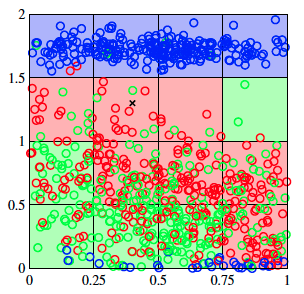
\includegraphics[scale=0.3]{images/pts.png}

\includegraphics[scale=0.4]{images/curse.png}
\end{center}

\end{frame}

% ========================================
\section{Оценка качетва классификации}
% ========================================

\begin{frame}{}

\begin{center}
\Large Оценка качетва классификации

\vspace{1em}

\includegraphics[scale=0.7]{images/learning.jpg}
\end{center}

\end{frame}

\begin{frame}{Как оценить различные модели?}

\begin{block}{Идея}
использовать долю неверно классифицированных объектов \\ (error rate)
\end{block}

\begin{alertblock}{Важное замечание}
error rate на обучающей выборке {\bf НЕ} является хорошим показателем качества модели
\end{alertblock}

\end{frame}

\begin{frame}{Решение 1: разделение выборки}

Делим обучающую выборку на {\bf тренировочную}, {\bf валидационную} и {\bf тестовую}

\begin{center}
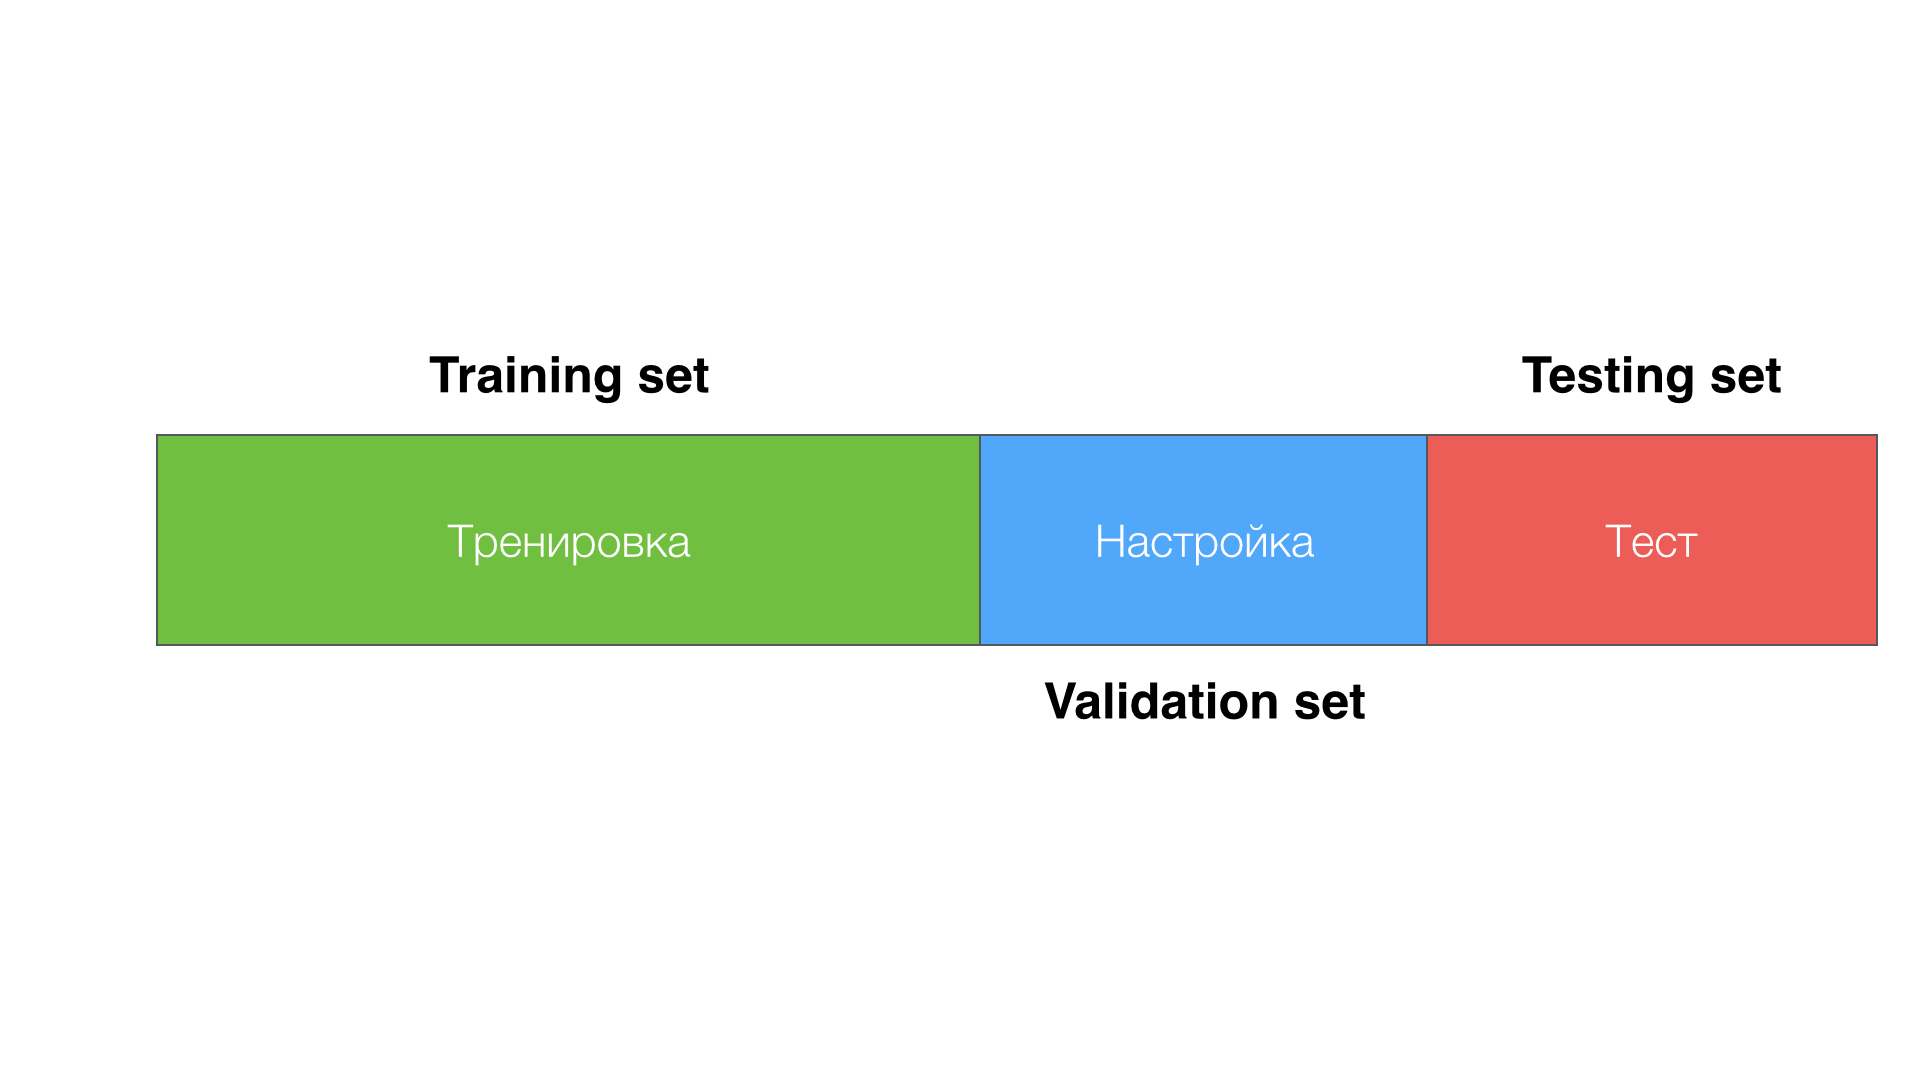
\includegraphics[scale=0.15]{images/vtt.png}
\end{center}
  
\end{frame}

\begin{frame}{Решение 2: скользящий контроль}

(n-times) (stratified) cross-validation

\begin{center}
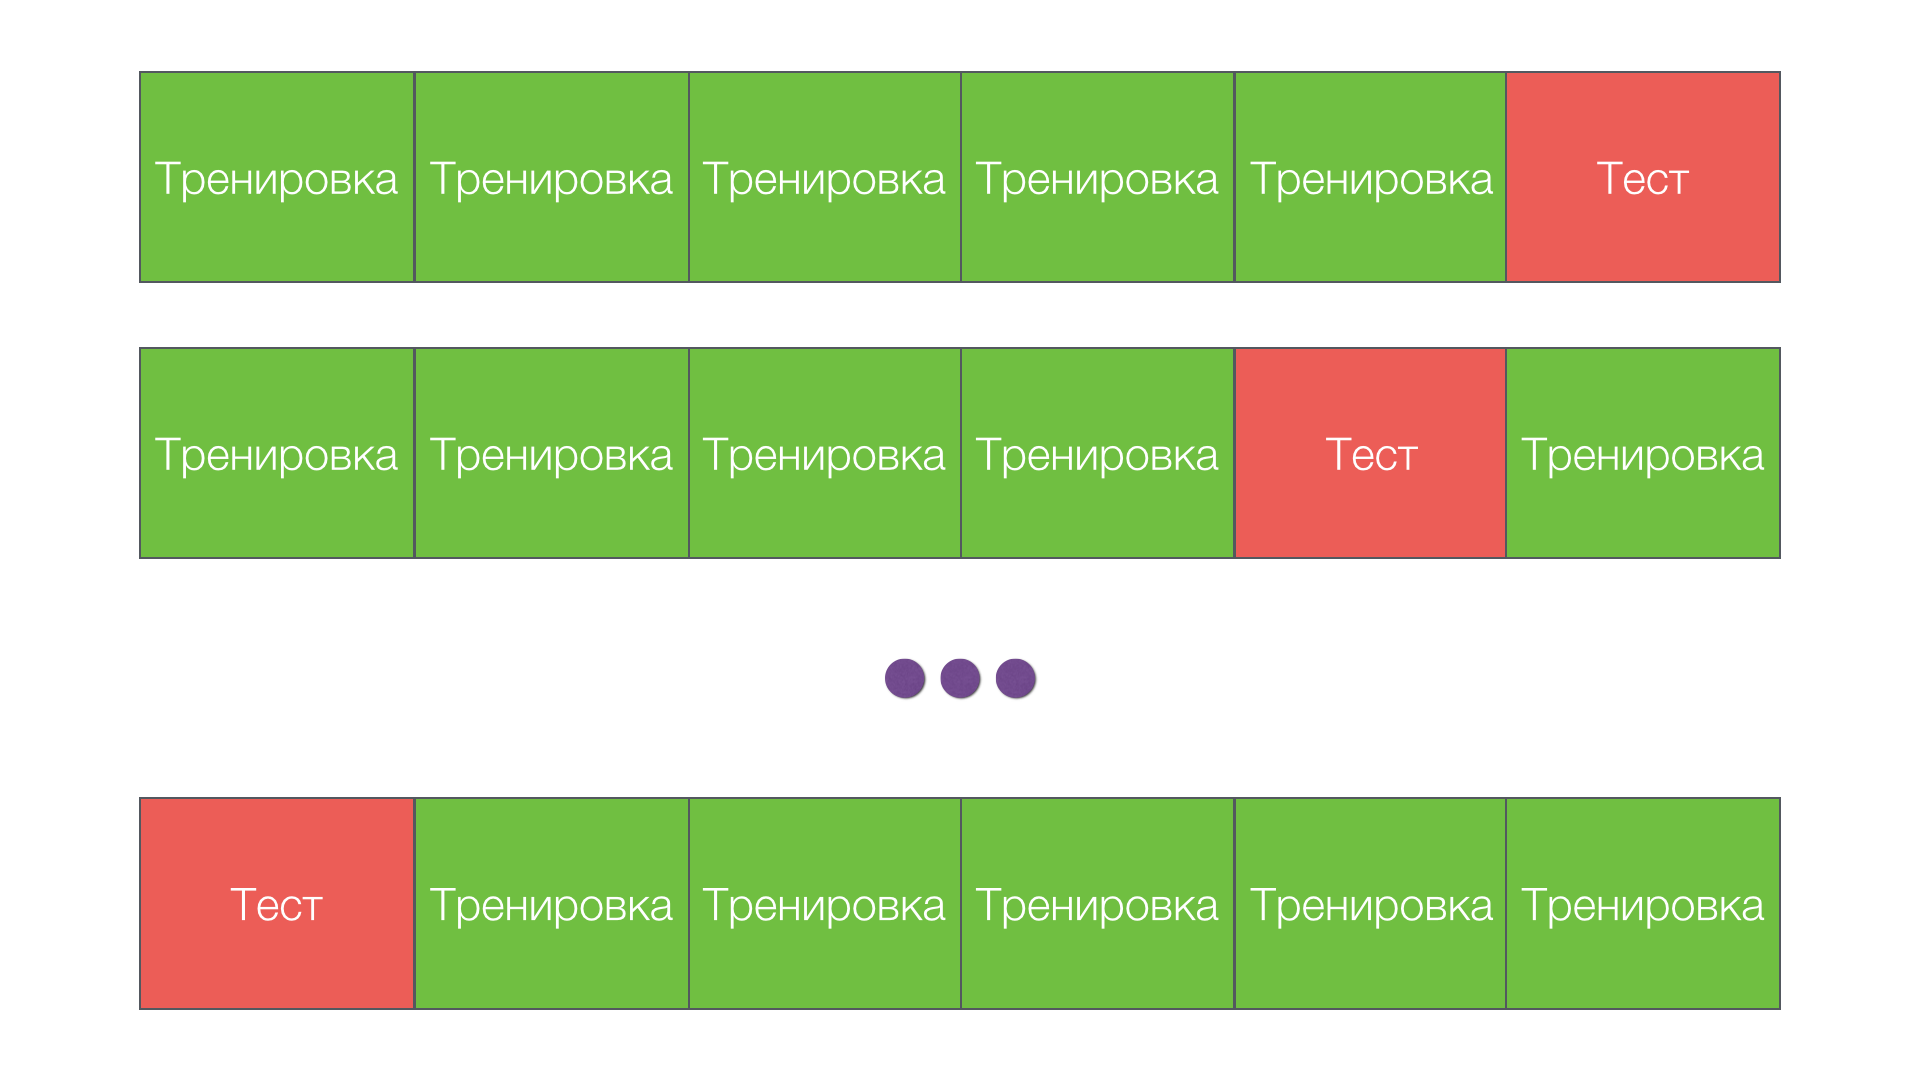
\includegraphics[scale=0.15]{images/cv.png}
\end{center}

частный случай: leave-one-out
  
\end{frame}

\begin{frame}{Решение 3: bootstrap}

выбираем в тренировочную выбоку $n$ объектов с возвращением

\begin{center}
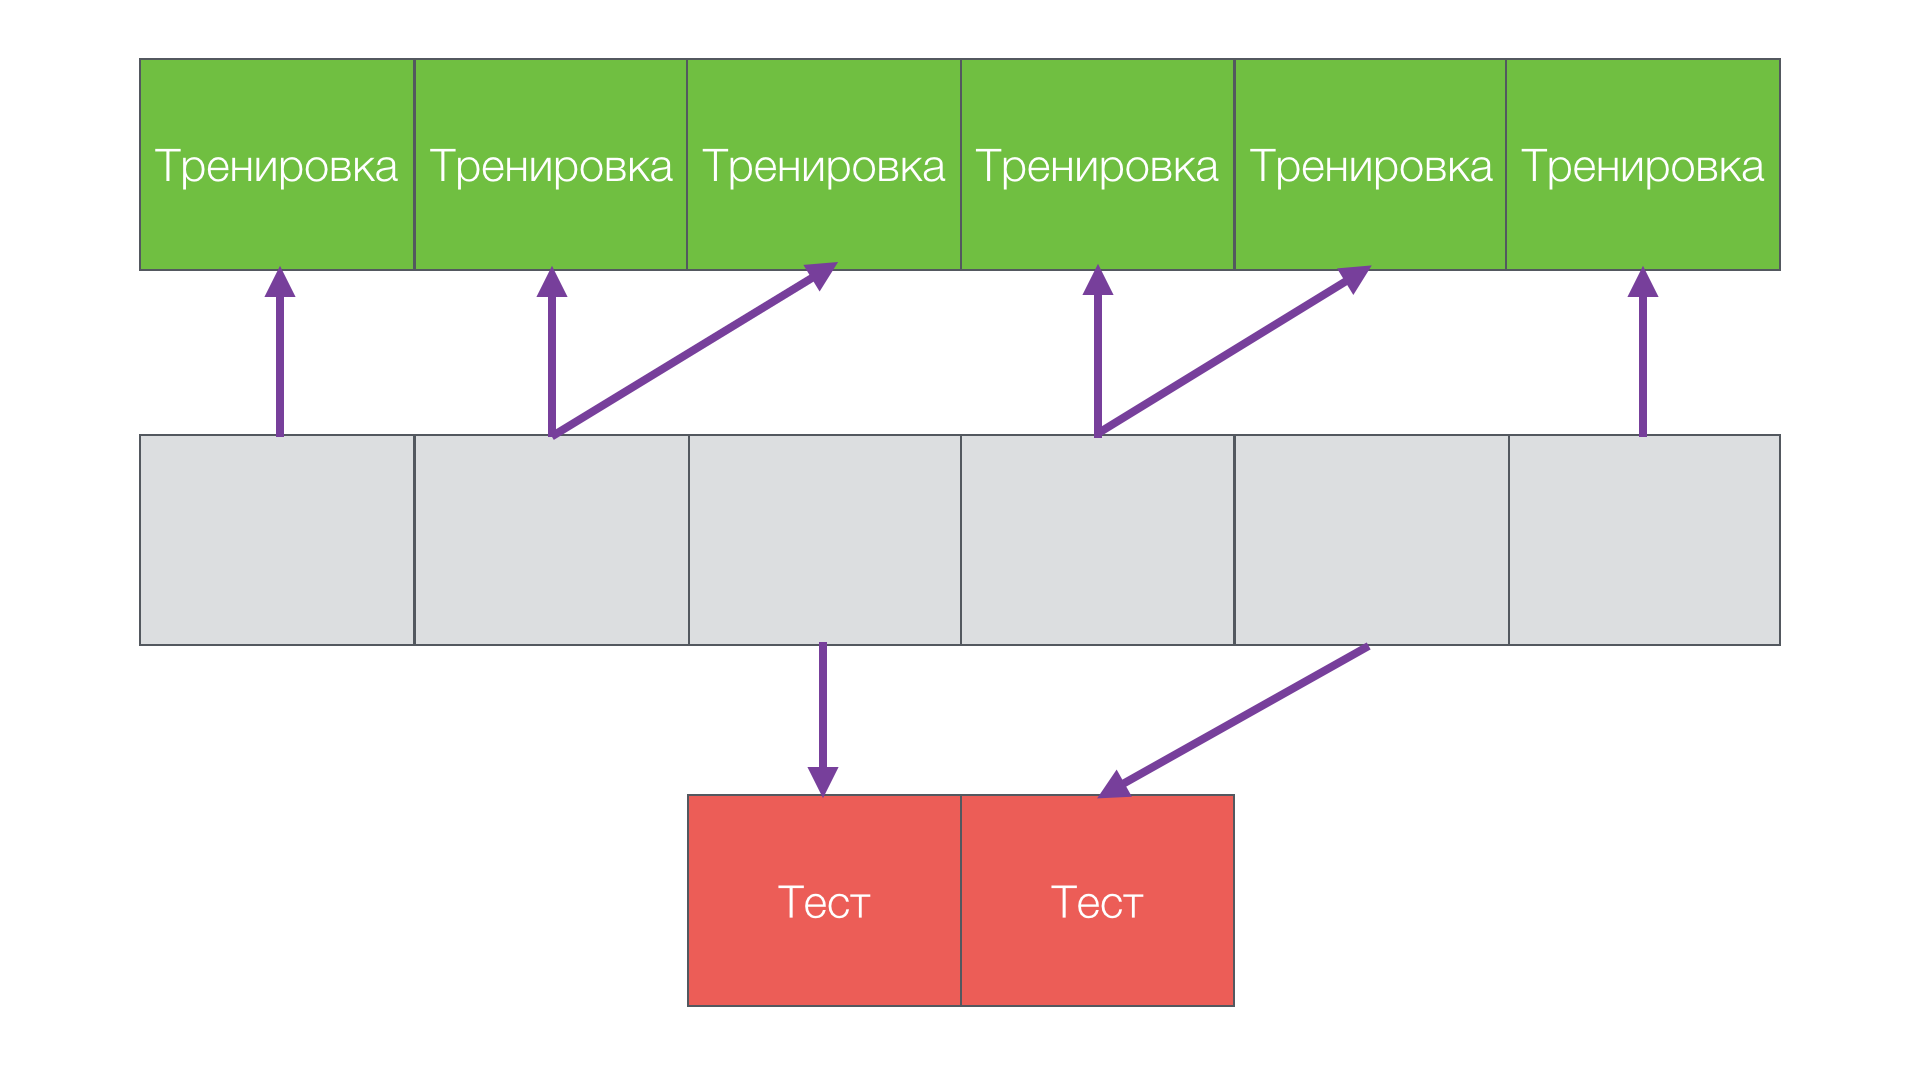
\includegraphics[scale=0.15]{images/boot.png}
\end{center}

упражнение: найти математическое ожидание размера тестовой выборки.
  
\end{frame}

\begin{frame}{Доверительный интервал для success rate}

\begin{small}

При тестировании на $N=100$ объектах было получено $25$ ошибок. Таким образом измеренная вероятность успеха (success rate) составила $f=0.75$. Найти доверительный интервал для действительной вероятности успеха c уровнем доверия $\alpha=0.8$. 

\begin{exampleblock}{Решение}
Пусть $p$ -- действительная вероятность успеха в испытаниях бернулли, тогда
\[
f \sim \mathcal{N}\left( p, p(1-p)/N \right).
\]
Воспользовавшись табличным значением $P(-z \leq \mathcal{N}(0,1) \leq z) = \alpha$, имеем
\[
P\left(-z \leq \frac{f-p}{\sqrt{p(1-p)/N}} \leq z \right) = \alpha,
\]
откуда
\[
p \in \left(f + \frac{z^2}{2N} \pm z \sqrt{\frac f N - \frac{f^2}{N}+\frac{z^2}{4N^2}} \right)/\left(1 + \frac {z^2}{N} \right) = [0.69, 0.80]
\]
\end{exampleblock}

\end{small}
  
\end{frame}

\begin{frame}{Метрики качества. Вероятностные модели.}

Пусть $y_i$ - действительный класс для объекта $\mathbf{x}_i$
\begin{itemize}
\item  Information loss 
\[
- \frac 1 N \sum_i \log_2 p(y_i | \mathbf{x}_i)
\]
\item Quadratic loss 
\[
\frac 1 N \sum_j (p(y_j | \mathbf{x}_i) - a_j(\mathbf{x}_i))^2,
\] 
где
\[
a_j(\mathbf{x}_i) = \begin{cases}
1, \;\text{если}\;C_j = y_i\\
0, \;\text{иначе}
\end{cases} 
\]
\end{itemize}

\end{frame}

\begin{frame}{Метрики качества. Функции решения.}

\begin{center}
\begin{tabular}{|c r | c c|}
\cline{3-4}
 \multicolumn{2}{c|}{} & \multicolumn{2}{c|}{Предсказанный} \\
 \cline{3-4}
 \multicolumn{2}{c|}{} & {\bf true} & {\bf false} \\
 \hline
 \multirow{2}{*}{Действительный} & \multicolumn{1}{|c|}{\bf true} & TP & FN \\
 & \multicolumn{1}{|c|}{\bf false}  & FP & TN \\
 \hline
\end{tabular}
\end{center}

\[
success\;rate = accuracy = \frac{TP + TN}{TP + FP + FN + TN}
\]
\[
recall = TPR = \frac{TP}{TP + FN};\;\;precision = \frac{TP}{TP + FP}
\]
\[
FPR = \frac{FP}{FP + TN}
\]
\[
affinity = lift = \frac{precision}{p}
\]

\end{frame}

\begin{frame}{Receiver Operating Characteristic}

\[
TPR = \frac{TP}{TP + FN};\;\;FPR = \frac{FP}{FP + TN}
\]

\begin{center}
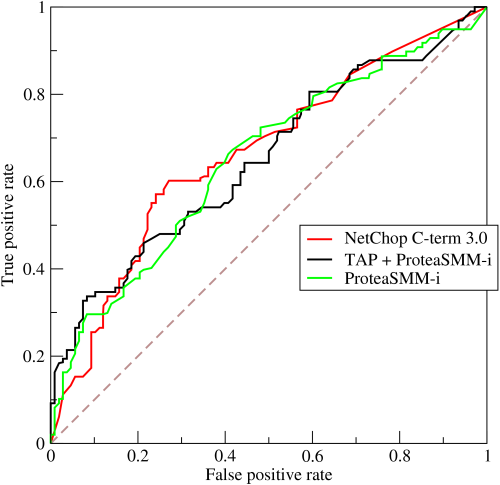
\includegraphics[scale=2.0]{images/roc.png}
\end{center}

\end{frame}

\begin{frame}{Упражнение}

\begin{exampleblock}{Простые классификаторы}
В генеральной совокупности существуют объекты 3 классов, вероятность появления которых $p_1 < p_2 < p_3$. Первый классификатор относит все объекты к классу с большей вероятностью (то есть к третьему). Второй классификатор случайно относит объект к одному из классов в соответствии с базовым распределением. Рассчитать precision и recall, которые эти классификаторы дают для каждого из 3 классов.
\end{exampleblock}

\end{frame}

\begin{frame}{Метрики качества. Регрессия}

\[
MSE = \frac 1 N \sum (h(\mathbf{x}_i) - y_i)^2, \;\; RMSE = \sqrt{MSE}
\]
\[
MAE =  \frac 1 N \sum |h(\mathbf{x}_i) - y_i|, \;\; RMAE = \sqrt{MAE}
\]
\[
RSE =  \frac{\sum (h(\mathbf{x}_i) - y_i)^2}{\sum (y_i - \bar{y})^2}
\]
\[
correlation = \frac{S_{hy}}{\sqrt{S_h S_y}};\;\; S_{yh} = \frac{\sum(h(i)-\overline{h(i)})(y_i - \bar y)}{N-1}
\]
\[
S_{h} = \frac{\sum(h(i)-\overline{h(i)})^2}{N-1};\;\;S_{y} = \frac{\sum(y_i - \bar y)^2}{N-1}
\]

\end{frame}

\begin{frame}{NFLT, MDL, AIC и все такое}

\begin{block}{No free lunch theorem}
Не существует единственной лучшей модели, решающей все задачи
\end{block}

\begin{block}{Minimum description length}
Лучшая гипотеза о данных -- та, которая ведет к самому краткому их описанию
\end{block}
\begin{block}{Akaike information criterion (AIC)}
\[
model = \arg\max	\ln p(\mathcal{D} | \theta_{ML}) - \|\theta\|
\]
\end{block}

\end{frame}

\begin{frame}[plain]
\begin{center}
{\Large Вопросы}
\end{center}
\end{frame}

\end{document}